%%%%%%%%%%%%%%%%%%%%%%%%%%%%%%%%%%%%%%%%%%%%%%%%%%%%%%%%%%%%%%%%%%%%%%%%%
\section{Inference Algorithm}  %%%%%%%%%%%%%%%%%%%%%%%%%%%%%%%%%%%%%%%%%%
\label{cr:sec:algorithm}

The maximizer of the log-posterior does not have a closed-form solution.
In the spirit of the algorithms of \citet{hunter2004mm} for variants of Luce's choice model, we develop a minorization-maximization (MM) algorithm.
Simply put, the algorithm iteratively refines an estimate of the maximizer by solving a sequence of surrogates of the log-posterior.
Using the inequality $\log x \le \log \tilde{x} + x/\tilde{x} - 1$ (with equality if and only if $x = \tilde{x}$), we can lower-bound the log-posterior~\eqref{cr:eq:logpost} by
\begin{align*}
&f^{(t)}(\bm{\lambda}) =
    \sum_{i = 1}^n \bigg[ (c^-_i + \alpha - 1) \log \lambda_i 
                         - c^+_i \bigg( \log\!\sum_{k \in N^+_i}\!\lambda^{(t)}_k
                                       +\frac{\sum_{k \in N^+_i}\!\lambda_k}{\sum_{k \in N^+_i}\!\lambda^{(t)}_k} -1 \bigg)
                         - \beta \lambda_i \bigg] + \kappa,
\end{align*}
with equality if and only if $\bm{\lambda} = \bm{\lambda}^{(t)}$.
Starting with an arbitrary $\bm{\lambda}^{(0)} \in \mathbf{R}^n_{>0}$, we repeatedly solve the optimization problem
\begin{align*}
\bm{\lambda}^{(t+1)} = \Argmax_{\bm{\lambda}} f^{(t)}(\bm{\lambda}).
\end{align*}
Unlike the maximization of the log-posterior, the surrogate optimization problem has a closed-form solution, obtained by setting $\nabla f^{(t)}$ to $\bm{0}$:
\begin{align}
\label{cr:eq:mmiter}
\lambda_i^{(t + 1)} = \frac{c^-_i + \alpha - 1}{\sum_{j \in N^-_i} \gamma_j^{(t)} + \beta},
\ \gamma_j^{(t)} = \frac{c^+_j}{\sum_{k \in N^+_j} \lambda_k^{(t)}}.
\end{align}
The iterates provably converge to the maximizer of~\eqref{cr:eq:logpost}, as shown by the following theorem.

\begin{theorem}
\label{cr:thm:mmconv}
Let $\bm{\lambda}^\star$ be the unique maximum a-posteriori estimate.
Then for any initial $\bm{\lambda}^{(0)} \in \mathbf{R}^n_{> 0}$ the sequence of iterates defined by~\eqref{cr:eq:mmiter} converges to $\bm{\lambda}^\star$.
\end{theorem}

Theorem~\ref{cr:thm:mmconv} follows from a standard result on the convergence of MM algorithms and uses the fact that the log-posterior increases after each iteration.
Furthermore, it is known that MM algorithms exhibit geometric convergence in a neighborhood of the maximizer \citep{lange2000optimization}.
A thorough investigation of the convergence properties is left for future work.

\begin{algorithm}[t]
  \caption{ChoiceRank}
  \label{cr:alg:choicerank}
  \begin{algorithmic}[1]
    \Require graph $G = (V, E)$, counts $\{ (c^-_i, c^+_i) \}$
    \State $\bm{\lambda} \gets [1, \ldots, 1]$
    \Repeat
      \State $\bm{z} \gets \bm{0}_n$
      \Comment{Recompute $\bm{\gamma}$}
      \OneLineFor{$(i, j) \in E$} $z_i \gets z_i + \lambda_j$
      \OneLineFor{$i \in V$} $\gamma_i \gets c^+_i / z_i$
      \State $\bm{z} \gets \bm{0}_n$
      \Comment{Recompute $\bm{\lambda}$}
      \OneLineFor{$(i, j) \in E$} $z_j \gets z_j + \gamma_i$
      \OneLineFor{$i \in V$} $\lambda_i \gets (c^-_i + \alpha - 1) / (z_i + \beta)$
    \Until $\bm{\lambda}$ has converged
  \end{algorithmic}
\end{algorithm}
%In practice, we notice that adding a little bit of regularization through the Gamma prior greatly improves convergence.

The structure of the updates in~\eqref{cr:eq:mmiter} leads to an extremely simple and efficient implementation, given in Algorithm~\ref{cr:alg:choicerank}: we call it ChoiceRank.
A graphical representation of an iteration from the perspective of a single node is given in Figure~\ref{cr:fig:msgpassing}.
Each iteration consists of two phases of message passing, with $\gamma_i$ flowing towards in-neighbors $N^-_i$, then $\lambda_i$ flowing towards out-neighbors $N^+_i$.
The updates to a node's state are a function of the sum of the messages.
As the algorithm does two passes over the edges and two passes over the vertices, an iteration takes $\BigO{m + n}$ time.
The edges can be processed in any order, and the algorithm maintains a state over only $\BigO{n}$ values associated with the vertices.
Furthermore, the algorithm can be conveniently expressed in the well-known vertex-centric programming model \citep{malewicz2010pregel}.
This makes it easy to implement ChoiceRank inside scalable, optimized graph-processing systems such as Apache Spark \citep{gonzalez2014graphx}.

\begin{figure}[t]
  \centering
  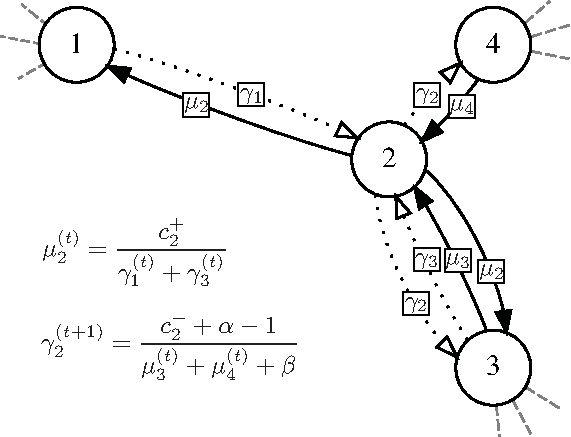
\includegraphics[width=0.5\linewidth]{cr-message-passing}
  \caption{One iteration of ChoiceRank from the perspective of node $2$.
  Messages flow in both directions along the edges of the graph $G$, first in the reverse direction (in dotted) then in the forward direction (in solid).}
  \label{cr:fig:msgpassing}
\end{figure}

\paragraph{EM Viewpoint}
The update~\eqref{cr:eq:mmiter} can also be explained from an expectation-maximization (EM) viewpoint, by introducing suitable latent variables \citep{caron2012efficient}.
This viewpoint enables a Gibbs sampler that can be used for Bayesian inference.
We present the EM derivation in Appendix~\ref{cr:app:algorithm}, but leave a study of fully Bayesian inference in the network choice model for future work.
